\chapter{Generelles}

\section{Referenzen}
\label{sec:referenzen}
\begin{wraptable}{r}{0.4\textwidth}
    \captionabove{Präfixe für Referenzen}
    \centering
    \begin{tblr}{ll}
        \toprule
        \textbf{Prefix} & \textbf{Bezeichnung} \\
        \midrule
        ch: & chapter \\
        sec: & section \\
        subsec: & subsection \\
        fig: & figure \\
        tab: & table \\
        eq: & equation \\
        code: & code listing \\
        itm: & enumerated list item \\
        alg: & algorithm \\
        app: & Anhang \\
        \bottomrule
    \end{tblr}
    \label{tab:praefixe-fuer-referenzen}
\end{wraptable}

Die Funktion \mintinline{latex}{\label{}} in \LaTeX dient dazu, Markierungen innerhalb des Textes zu setzen, auf die später mithilfe von Referenzen zugegriffen werden kann. Dies ist besonders nützlich, um Verweise auf Abschnitte, Kapitel, Gleichungen, Abbildungen oder Tabellen innerhalb eines \LaTeX-Dokuments zu erstellen. Label sollten für die einfachere Zuordnung aussagekräftig beschrieben sein. So bietet es sich zum Beispiel an für Kapitel (engl. chapter) \texttt{ch:} an den Anfang des Labels zu schreiben, für Abschnitte (engl. section) \texttt{sec:}, usw (vgl. \autoref{tab:praefixe-fuer-referenzen}). Indem man ein Label mit einem eindeutigen Namen an der gewünschten Stelle platziert, kann man später im Text mithilfe von \mintinline{latex}{\autoref{}} auf dieses Label verweisen, um automatisch die Bezeichnung inkl. Nummer einzufügen. Dies erleichtert die Aktualisierung von Referenzen, wenn sich die Nummerierung oder Anordnung im Dokument ändert, da LaTeX automatisch die korrekten Nummern aktualisiert.

\begin{showcode}{latex}
    \subsection{Beispiel für Referenzen}
    \label{subsec:beispiel-fuer-referenzen}

    Wie in \autoref{subsec:beispiel-fuer-referenzen} beschrieben…
\end{showcode}

Bei der Vergabe eindeutiger Bezeichner für die Referenzierung sollte darauf geachtet werden, dass lediglich ASCII-Zeichen verwendet werden. Je nach Kodierung der Quelldatei können Sonderzeichen sonst zu Fehlermeldungen führen.

\subsection{Weitere Referenzmöglichkeiten}

\begin{description}
    \item[\mintinline{latex}{\label{}}] Gibt dem zu referenzierenden Objekt einen Namen, auf den später referenziert werden kann.
    \item[\mintinline{latex}{\ref{}}] Referenziert auf das Objekt und gibt nur die Nummer für dieses Objekt zurück (sollte nur selten verwendet werden).
    \item[\mintinline{latex}{\pageref{}}] Gibt die Seitenzahl des referenzierten Objektes zurück.
    \item[\mintinline{latex}{\autoref{}}]\label{itm:autoref} Referenziert auf das Objekt mit der Bezeichnung und der Nummer. \textbf{Dies ist die präferierte Variante.}
    \item[\mintinline{latex}{\nameref{}}] Gibt den Inhalt des naheliegendsten relevanten Objekt zurück. So wird bei einer Überschrift diese zurückgegeben, aber für ein Bild der Inhalt der Bildunterschrift.
\end{description}

\section{Fließumgebungen}
\label{sec:fliessumgebungen}
Fließumgebungen (engl. floats) sind ein wichtiger Bestandteil von \LaTeX-Dokumenten, um Grafiken, Abbildungen, Tabellen und ähnliche Inhalte flexibel und ästhetisch ansprechend im Layout zu platzieren. Durch die Verwendung von Fließumgebungen können diese Elemente automatisch an geeigneten Stellen im Text platziert werden, um den Lesefluss nicht zu unterbrechen. Innerhalb von Fließumgebungen kann der Befehl \mintinline{latex}{\caption{}} verwendet werden, um Bild- oder Tabellenbeschriftungen hinzuzufügen, sowie der Befehl \mintinline{latex}{\label} (siehe \autoref{sec:referenzen}), um Labels für Referenzen festzulegen. 

Trotz der automatischen Platzierung von Fließumgebungen in \LaTeX gibt es Situationen, in denen eine manuelle Kontrolle über die Positionierung erforderlich ist. \LaTeX bietet Optionen, um Fließumgebungen an bestimmten Stellen im Text zu platzieren. Die Option \texttt{[h]} (here) erlaubt eine Platzierung am Ort des Befehls im Text. \texttt{[t]} (top) platziert die Umgebung oben auf einer Seite, \texttt{[b]} (bottom) unten auf einer Seite und \texttt{[p]} (page) auf einer separaten Seite nur für Fließumgebungen. Soll die Fließumgebung fix an die vom Autor angegebene Stelle platziert werden, kann die Option \texttt{[H]} (Here!) verwendet werden. Diese Option zwingt \LaTeX zur Positionierung an der angegebenen Stelle. Manuelle Positionierungsoptionen sollten jedoch sparsam verwendet werden, da sie die typografische Ästhetik beeinträchtigen könnten.

\subsection{Beschriftungen}
\label{sec:beschriftungen}
In \LaTeX ermöglicht der Befehl \mintinline{latex}{\caption{}} das Hinzufügen von Beschriftungen zu Fließumgebungen. Diese Beschriftungen bieten eine kurze Erklärung oder Bezeichnung für das jeweilige Element. Beschriftungen sind hilfreich, um den Inhalt für den Leser zu erläutern und in den Kontext des Dokuments zu setzen. Darüber hinaus generiert \LaTeX automatisch die richtige Nummerierung für Abbildungen und Tabellen, was die Konsistenz und Verwaltung erleichtert. Durch die Kombination von \mintinline{latex}{\caption{}} mit \mintinline{latex}{\label{}} können Sie außerdem Referenzen zu diesen Elementen erstellen, die im Text automatisch die korrekte Nummer und Bezeichnung anzeigen (vgl. \autoref{itm:autoref}). Mit dem Befehl \mintinline{latex}{\captionof{float}{}} können Beschriftungen auch außerhalb von Fließumgebungen für bestimmte Elemente gesetzt werden. 

Für Tabellen werden in wissenschaftlichen Artikeln die Beschriftungen häufig oberhalb des Elements gesetzt, da die Beschriftung unterhalb der Tabelle bei langen Tabellen zu spät gelesen wird. Bei Bildern hingegen sind die Beschriftungen unterhalb des Elements. Da die Formatierung von \LaTeX diesen Unterschied bei Tabellen nicht berücksichtigt existiert in diesem Dokument der Befehl \mintinline{latex}{\captionabove{}}, welcher den Abstand zwischen Beschriftung und Tabelle korrigiert.

\subsection{Zentrierung}
Es ist oft sinnvoll, Fließumgebungen wie Tabellen oder Bilder zu zentrieren, insbesondere wenn sie nicht die volle Textbreite ausfüllen. Dies trägt zur ästhetischen Gestaltung des Dokuments bei und sorgt dafür, dass diese Elemente optisch ausgerichtet und präsentiert werden. Es gibt zwei gängige Möglichkeiten, dies in \LaTeX zu erreichen.

Die erste Möglichkeit ist die Verwendung der \texttt{center}-Umgebung, welche \textbf{keine} Fließumgebung darstellt:

\begin{showcode}{latex}
    \begin{center}
        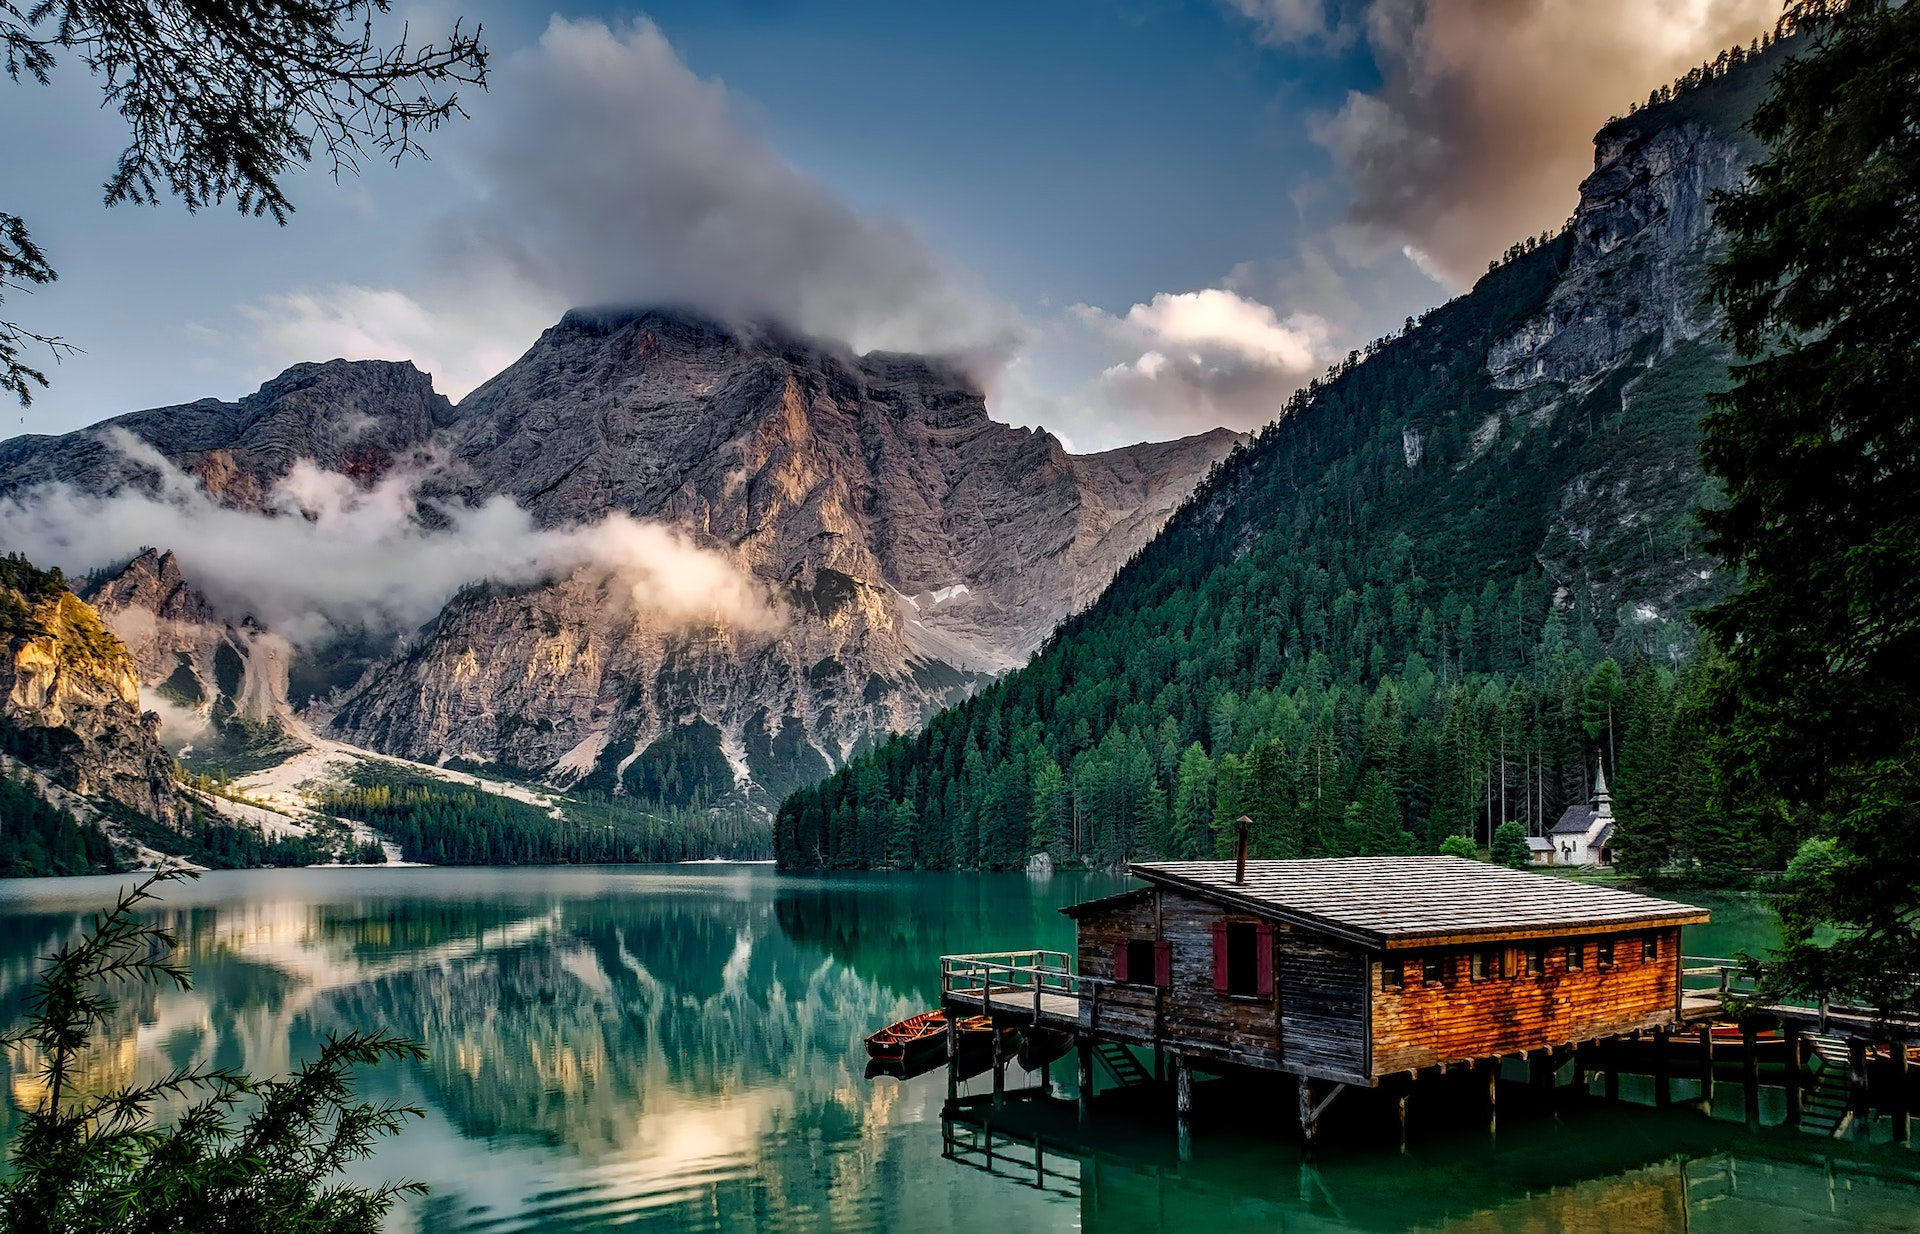
\includegraphics[width=0.4\columnwidth]{assets/images/bilder/pexels-pixabay-147411.jpg}
        \captionof{figure}{Beschriftung des Bildes}
    \end{center}
\end{showcode}

Die zweite Möglichkeit ist die Verwendung des Befehls \mintinline{latex}{\centering} innerhalb einer Fließumgebung:

\begin{showcase}
    \begin{code}{latex}
        \begin{figure}
            \centering
            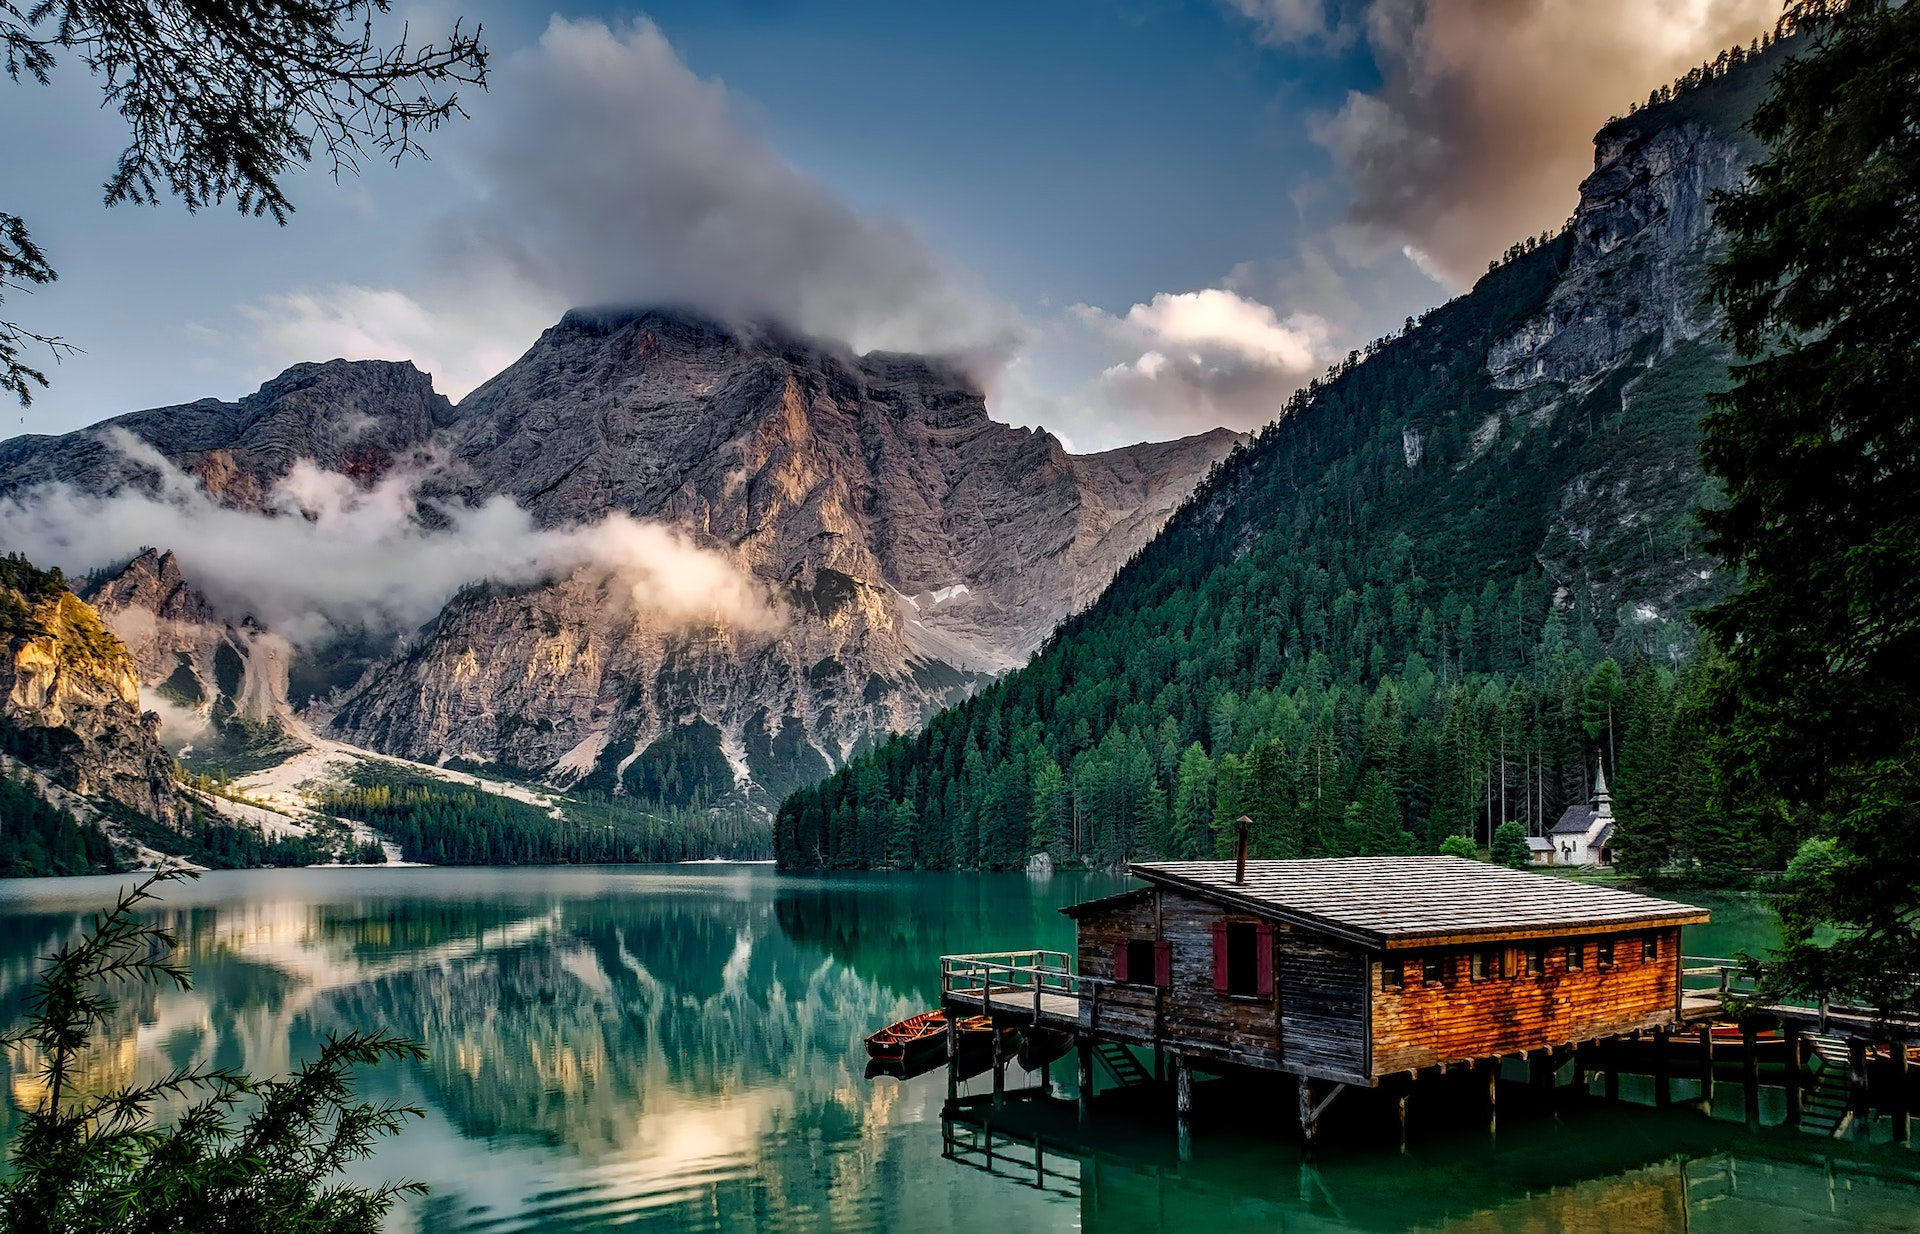
\includegraphics[width=0.4\columnwidth]{assets/images/bilder/pexels-pixabay-147411.jpg}
            \caption{Beschriftung des Bildes}
        \end{figure}
    \end{code}
    \tcblower
    \begin{center}
        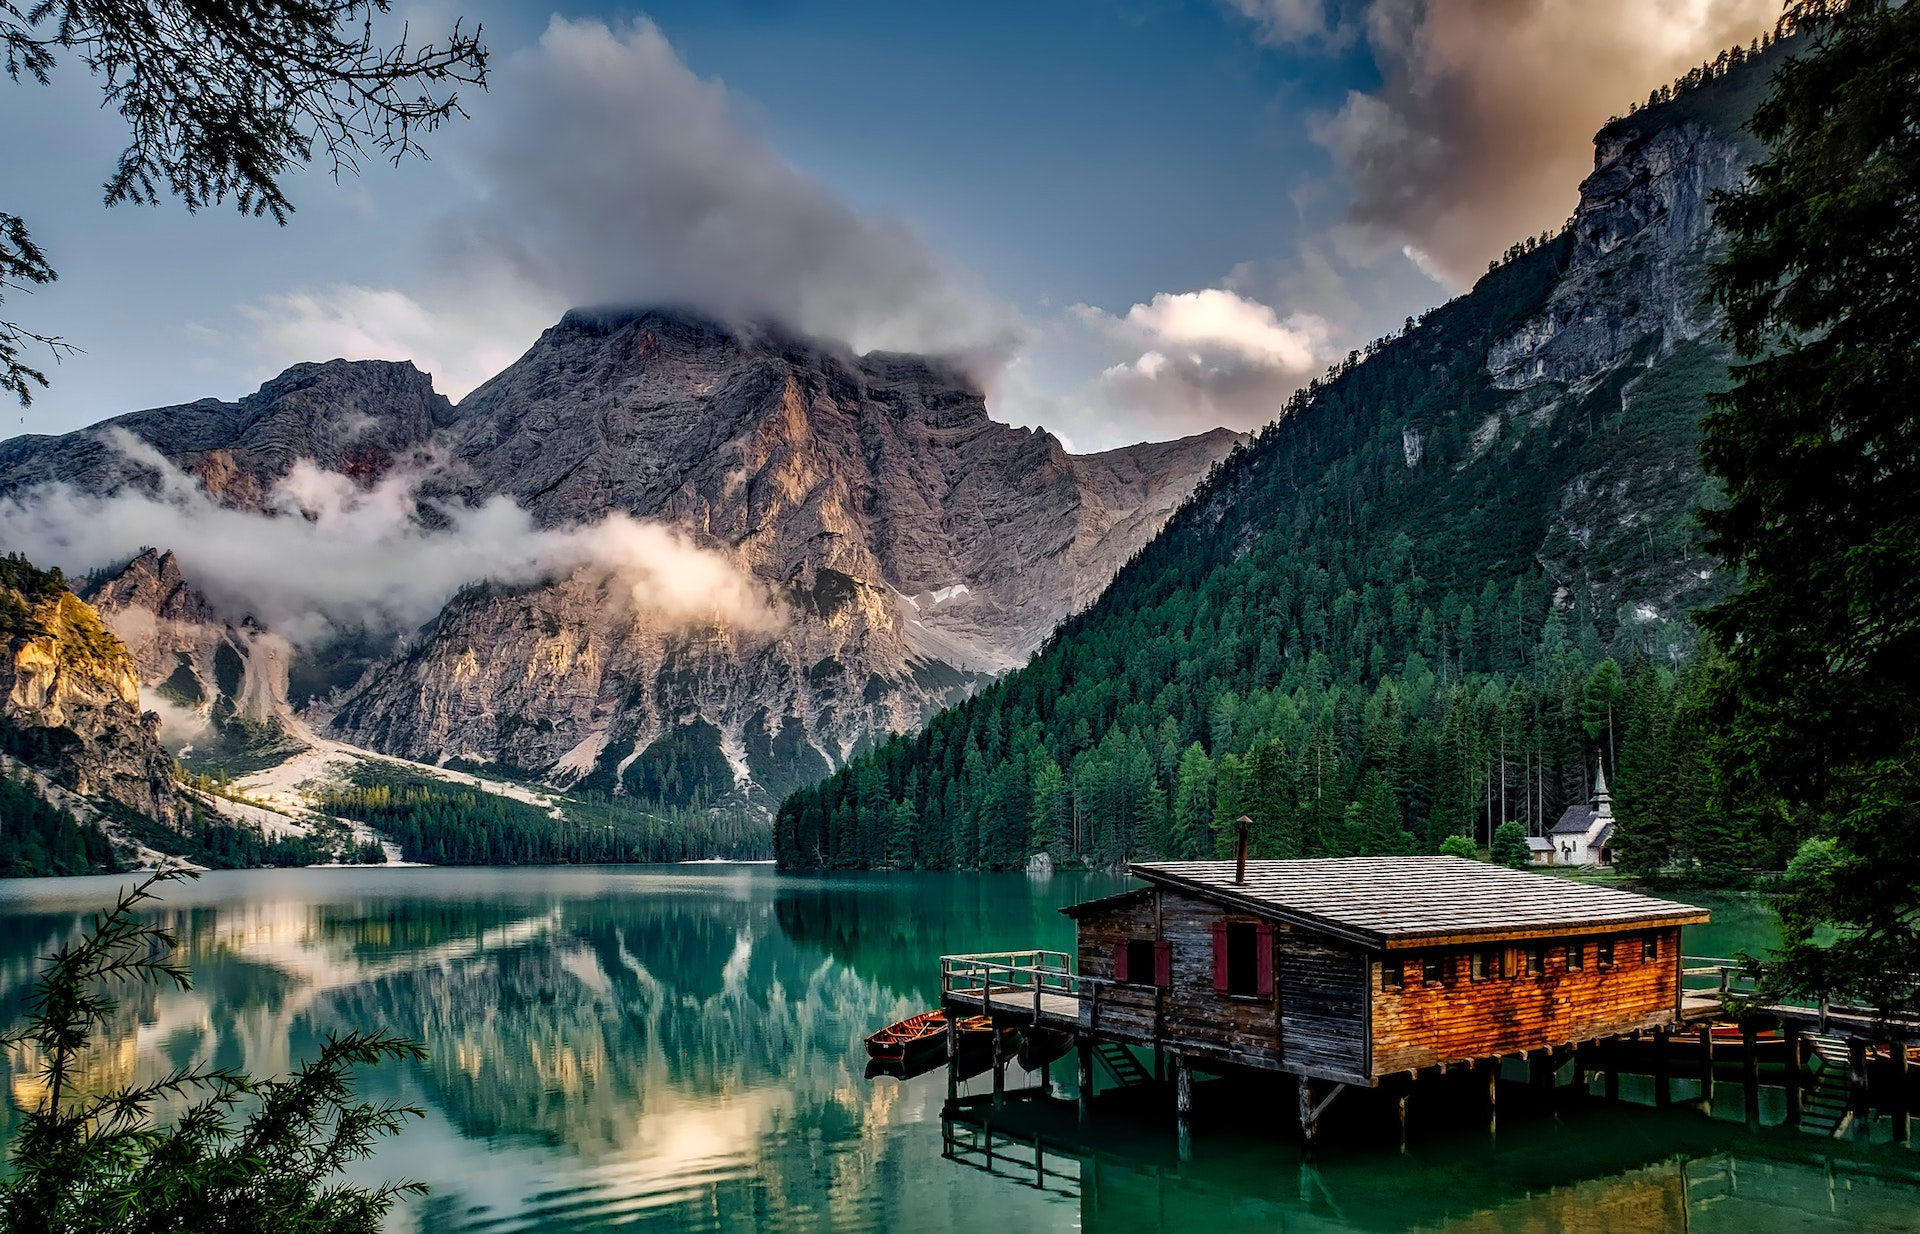
\includegraphics[width=0.4\columnwidth]{assets/images/bilder/pexels-pixabay-147411.jpg}
        \captionof{figure}{Beschriftung des Bildes}
    \end{center}
\end{showcase}

Beide Methoden zentrieren den Inhalt horizontal im Dokument. Mit der \texttt{center}-Umgebung erhalten wir jedoch keine Fließumgebung, weshalb wir für eine Beschriftung des Bildes den Befehl \mintinline{latex}{\captionof{figure}{}} verwenden müssen. Wie in \autoref{sec:fliessumgebungen} beschrieben ist auch keine optimierte Positionierung des Elements durch \LaTeX möglich.